\documentclass{article}

% Dùng pdflatex (Overleaf default)
\usepackage[final]{neurips_2026}
\usepackage[utf8]{inputenc}
\usepackage[T5]{fontenc}
\usepackage[vietnamese]{babel}

\usepackage{amsmath}
\usepackage{graphicx}
\usepackage{booktabs}
\usepackage{caption}
\usepackage{subcaption}
\usepackage{hyperref}
\usepackage{microtype}

\graphicspath{{./}}

\title{Dự báo Doanh thu Thương mại Điện tử:\\
Phân tích Sụp đổ 2019 và Phục hồi 2023--2024}

\author{
  Nhóm Deus x Machina \\
  VinUniversity \\
  \texttt{dungroi19@gmail.com} \quad
  \href{https://github.com/graviton711/datathon\_main}{github.com/graviton711/datathon\_main}
}

\begin{document}
\maketitle

% =========================================================
\section{Giới thiệu}
% =========================================================

Dự báo doanh thu thương mại điện tử (TMĐT) ngày nay đòi hỏi độ chính xác cao đến từng ngày để tối ưu tồn kho và vận hành logistics. Tuy nhiên, các chuỗi thời gian thực tế thường chứa các đứt gãy cấu trúc (structural breaks) khiến việc học từ dữ liệu lịch sử trở nên khó khăn. Bộ dữ liệu trong nghiên cứu này (Bảng~\ref{tab:data}) ghi lại 10 năm hoạt động của một doanh nghiệp Việt Nam, với biến cố sụt giảm gần 40\% lượng đơn hàng vào năm 2019 do sự cố mất niềm tin của khách hàng (Trust Collapse). Thách thức chính là xây dựng một hệ thống dự báo có khả năng thích nghi với bối cảnh thị trường mới (regime) mà không bị nhiễu bởi quy mô quá lớn của giai đoạn cũ, đồng thời kiểm soát sai số tích lũy trong chu kỳ dự báo (horizon) dài 548 ngày.

\begin{table}[h]
\centering
\caption{Tổng quan bộ dữ liệu (14 bảng, 4 lớp).}
\label{tab:data}
\small\setlength\tabcolsep{4pt}
\begin{tabular}{llll}
\toprule
\textbf{Lớp} & \textbf{Bảng chính} & \textbf{Giai đoạn} & \textbf{Quy mô} \\
\midrule
Master      & products, customers, promotions & --        & 2,412 sản phẩm \\
Transaction & orders, order\_items, payments  & 2012--2022 & $\sim$647k đơn hàng \\
Analytical  & sales.csv, sample\_submission   & 2012--2024 & 3{,}833 ngày \\
Operational & inventory, web\_traffic         & 2012--2022 & Tháng/ngày \\
\bottomrule
\end{tabular}
\end{table}

Để giải quyết bài toán này, chúng tôi đề xuất hệ thống dự báo \emph{Recursive LightGBM} kết hợp
kỹ thuật \emph{Stationary Normalization} để xử lý đứt gãy cấu trúc. Mô hình đạt
\textbf{MAE = 684{,}330} trên tập đánh giá chéo (Weighted CV) -- cải thiện 19.2\% so với
phương pháp cơ sở (Last Year Naive Baseline) và ngăn chặn tuyệt đối rò rỉ dữ liệu.

% =========================================================
\section{Phân tích Dữ liệu (EDA)}
% =========================================================

\subsection{Mô tả -- \textit{Chuyện gì đã xảy ra?}}

\begin{figure}[h]
  \centering
  
\includegraphics[width=0.85\linewidth]{18_regional_order_trend}
  \caption{Xu hướng đơn hàng 2012--2022 theo vùng địa lý. Cả ba vùng
    East, Central, West đều sụt giảm \textbf{đồng thời} từ 2018,
    loại trừ khả năng do vấn đề logistics hay giao hàng cục bộ.}
  \label{fig:regional}
\end{figure}

Giai đoạn 2012--2018 chứng kiến sự tăng trưởng nóng, trước khi doanh số
đột ngột bốc hơi vào năm 2019. Tỷ lệ huỷ đơn luôn duy trì ổn định ở mức 9.2\%, không
đủ để giải thích nguyên nhân của mức giảm 40\% này. Đáng chú ý, gần 39\% đơn hàng phải dùng
đến khuyến mãi, cho thấy doanh nghiệp đã nỗ lực dùng chiết khấu để
níu kéo doanh thu. Tỷ trọng giá vốn hàng bán trên doanh thu (COGS/Revenue) cũng có
dấu hiệu biến động mạnh qua các năm, đòi hỏi một quy trình dự báo tách biệt cho chi phí này.

\subsection{Chẩn đoán -- \textit{Tại sao lại xảy ra?}}

\begin{figure}[h]
  \centering
  \begin{subfigure}[b]{0.49\linewidth}
    
\includegraphics[width=\linewidth]{12_traffic_conversion}
    \caption{Lượt truy cập tăng, tỷ lệ chuyển đổi giảm từ 1.2\% xuống dưới 0.4\%.}
    \label{fig:conversion}
  \end{subfigure}
  \hfill
  \begin{subfigure}[b]{0.49\linewidth}
    
\includegraphics[width=\linewidth]{16_retention_heatmap}
    \caption{Tỷ lệ giữ chân khách ở năm thứ 2 rớt từ 64.7\% xuống 9.4\%.}
    \label{fig:retention}
  \end{subfigure}
  \caption{Hai bằng chứng cốt lõi của sự mất niềm tin (Trust Collapse): lưu lượng truy cập
    không thiếu nhưng khách không chốt đơn (trái); mua rồi thì không quay lại (phải).}
  \label{fig:diagnostic}
\end{figure}

Về mặt chuỗi cung ứng, tỷ lệ lấp đầy đơn hàng (fill rate) duy trì
ở mức $\sim$100\% suốt năm 2019. Điều này loại trừ nguyên nhân thiếu hụt hàng hóa. 
Hình~\ref{fig:conversion} cho thấy lưu lượng truy cập thực ra
\emph{tăng} trong cùng kỳ, nhưng tỷ lệ chuyển đổi (Conversion Rate) lại rơi tự do từ 1.2\% xuống dưới 0.4\%.
Khách vào xem nhiều nhưng ít chốt đơn -- đây là minh chứng rõ ràng của sự sụt giảm niềm tin
vào chất lượng sản phẩm.

Phân tích lý do trả hàng làm sáng tỏ vấn đề: 52.6\% lượng hàng bị trả về do
sai kích cỡ (\textit{wrong\_size}) hoặc không giống mô tả (\textit{not\_as\_described}). Kết hợp với
Hình~\ref{fig:retention} -- tỷ lệ khách hàng quay lại mua vào năm thứ hai giảm từ 64.7\% (nhóm khách hàng năm 2012)
xuống mức báo động 9.4\% (nhóm khách hàng năm 2018) -- chúng tôi kết luận đây
là vòng xoáy "đốt tiền tìm khách rồi mất trắng" (burn-and-churn): khách mua lần đầu, nhận hàng
không đúng kỳ vọng, trả hàng và vĩnh viễn không quay lại.

\subsection{Dự báo và Đề xuất -- \textit{Điều gì xảy ra tiếp theo?}}

\textbf{Lộ trình phục hồi.}
Rating trung bình duy trì ổn định quanh mức 3.9 suốt giai đoạn sụt giảm doanh số. Tuy nhiên, chu kỳ mua lặp lại trung vị dài $\sim$144 ngày cho thấy một sự cố về niềm tin có thể mất nhiều tháng để phản ánh hết lên doanh số.
Mô hình dự báo tổng doanh thu năm 2023 đạt \textbf{1.22 tỷ VND} ($+$4.1\% so với 2022),
với cao điểm vào Quý 2 (tháng 5--6, $\sim$5.1 triệu/ngày) và dịp Tết tháng 2 ($\sim$3.3 triệu/ngày).
Tháng 7 là vùng trũng doanh thu ($\sim$3.4 triệu/ngày, giảm 32\% so với đỉnh điểm tháng 6),
tạo thời điểm vàng để tái cơ cấu tồn kho.

\textbf{Ba đề xuất hành động ưu tiên:}
\begin{itemize}
  \item \textbf{(1) Cải thiện bảng hướng dẫn chọn size.}
    52.6\% lý do hoàn trả xuất phát từ việc sai kích cỡ và mô tả không đúng,
    chủ yếu ở nhóm hàng Streetwear (size XL và S). Tác động trực tiếp của việc khắc phục lỗi này là tiết kiệm được
    gần 19 triệu VND/năm chi phí hoàn tiền. Quan trọng hơn, đây chính là nguyên nhân gốc rễ làm sụp đổ niềm tin khách hàng 
    khiến tỷ lệ giữ chân khách năm thứ 2 rớt thảm hại. Chuẩn hóa kích cỡ là điều kiện tiên quyết.
  \item \textbf{(2) Tiếp thị lại (Retargeting) tập khách hàng cũ 2016--2018}
    \textit{(Chỉ thực hiện sau khi đã hoàn thành bước (1)).}
    Có 10,326 khách hàng "ngủ đông" (từng mua nhưng không có đơn mới từ 2019), với giá trị đơn hàng trung bình (AOV) $\sim$22,000 VND.
    Việc tiếp cận lại nhóm này sẽ tiết kiệm chi phí hơn so với việc tìm kiếm khách hàng mới. Tuy nhiên, nếu lỗi kích cỡ chưa được khắc phục, 
    khách sẽ tiếp tục rời bỏ sau lần mua lại đầu tiên, gây lãng phí toàn bộ ngân sách tiếp thị.
  \item \textbf{(3) Phân bổ lại tồn kho theo kích cỡ.}
    Dữ liệu chỉ ra một "Nghịch lý tồn kho": Xác suất hết hàng lên tới $\sim$67\% xảy ra
    đồng đều ở \textit{tất cả} các danh mục sản phẩm, mặc dù lượng hàng lưu kho đủ bán trong hàng trăm đến hàng nghìn ngày.
    Vấn đề nằm ở sự mất cân đối giữa các biến thể sản phẩm cụ thể (SKU) chứ không phải thiếu tổng lượng hàng.
    Cần ưu tiên tái cân bằng các mã sản phẩm (SKU) Streetwear (nhóm có biên lợi nhuận 21.5\% và rating ổn định $\sim$3.9)
    theo đúng nhu cầu kích cỡ thực tế vào thời điểm thấp điểm tháng 7.
\end{itemize}

% =========================================================
\section{Mô hình Dự báo}
% =========================================================

\subsection{Đặc trưng và Kiến trúc}

\begin{table}[h]
\centering
\caption{Nhóm đặc trưng đầu vào.}
\label{tab:features}
\small\setlength\tabcolsep{4pt}
\begin{tabular}{lll}
\toprule
\textbf{Nhóm} & \textbf{Đặc trưng} & \textbf{Vai trò} \\
\midrule
Calendar    & dow, month, day\_of\_month  & Chu kỳ ngày \\
Lag/Rolling & lag\_1, lag\_7, roll\_7/30 & Momentum ngắn hạn \\
Sự kiện     & is\_tet, is\_payday, is\_event & Đỉnh bất thường \\
Danh mục    & share\_streetwear, \ldots   & Cơ cấu doanh thu \\
Momentum    & prev\_q4\_momentum          & Xu hướng dài hạn \\
\bottomrule
\end{tabular}
\end{table}

Để kiểm soát rủi ro rò rỉ dữ liệu, hệ thống tuân thủ quy tắc phân chia dữ liệu ngặt nghèo theo thời gian (\textit{strict temporal split}), chỉ sử dụng các đặc trưng độ trễ (lags) khả dụng tính đến thời điểm $t$.

\textbf{Chuẩn hóa tĩnh (Stationary Normalization).}
Bộ dữ liệu chịu một đứt gãy cấu trúc năm 2019 khiến phân phối doanh thu
thay đổi vĩnh viễn ($\mu_{\text{2012--2018}} \approx 1.6\times\mu_{\text{2019+}}$).
Nếu huấn luyện trực tiếp trên giá trị doanh thu tuyệt đối, mô hình khi tối ưu trên
giai đoạn cũ sẽ dự báo vọt lên (over-predict) toàn bộ chu kỳ 2023--2024.
Giải pháp: áp dụng kỹ thuật \textit{Stationary Normalization} \cite{stationary}, chuẩn hóa mục tiêu dự báo theo trung vị (median) của năm đó:
\begin{equation}
  \tilde{r}_t = \frac{\text{Revenue}_t}{\hat{\mu}_{\text{year}(t)}},
  \quad \hat{\mu}_{\text{year}} = \operatorname{median}_{d\in\text{year}}(\text{Revenue}_d),
\end{equation}
Cách này chuyển bài toán từ ``dự báo mức doanh thu tuyệt đối'' sang
``dự báo vị trí tương đối trong năm''.
Các đặc trưng độ trễ cũng được chia cùng tỷ lệ này để
giữ tính đồng nhất về mặt không gian dữ liệu.
Khi đưa vào dự báo thực tế (inference), giá trị được tính ngược lại bằng $\hat{r}_t = \tilde{r}_t \times M_t$
trong đó $M_t$ là projected median của năm dự báo, tính từ momentum tăng trưởng
(Blended Category Momentum). Cơ chế này cho phép mô hình học pattern hình dạng chu kỳ mà không bị nhiễu bởi chênh lệch quy mô tuyệt đối giữa hai regime, đạt mức MAE ổn định $\sim$684k trên toàn bộ các fold kiểm thử.

\textbf{Kiến trúc dự báo cuốn chiếu (Recursive).}
Sau 2019, tính mùa vụ trở nên khó lường hơn và các biến số lag\_1/lag\_7/roll\_7
vươn lên chiếm 3 vị trí đầu về mức độ quan trọng. Điều này cho thấy đà tăng trưởng ngắn hạn (momentum) quan
trọng hơn mùa vụ cố định, là cơ sở để chọn kiến trúc dự báo cuốn chiếu thay vì dự báo trực tiếp (Direct).
Vấn đề sai số tích lũy (error accumulation) qua 548 ngày được kiểm soát bằng \textbf{Hệ số giảm chấn (Damped Multiplier)}
$g^{(k)}=g^{\delta_k}$, với thông số suy giảm ($\delta_1 = 0.85$, $\delta_2 = 0.3$) được tối ưu hóa qua tập kiểm thử; các biến độ trễ được chuẩn hóa theo $M_t$
nên sai số tuyệt đối không bị khuếch đại sang bước tiếp theo.
Chi phí giá vốn (COGS) được dự báo qua tỷ lệ $\rho_t=\text{COGS}_t/(\text{Revenue}_t+\varepsilon)$
thay vì dự báo thẳng ra giá trị tuyệt đối; mô hình cũng áp dụng trọng số tập trung vào dữ liệu từ 2019 trở đi (bối cảnh thị trường hiện hành).

Bốn cơ chế then chốt trong vòng lặp dự báo:
\textbf{(i) Hệ số đà tăng trưởng tổng hợp (Blended Category Momentum)} -- mỗi ngày $t$ tính hệ số
$m_t = \sum_c s_{c,t} \cdot \mu_c$ (tỷ trọng danh mục nhân đà tăng trưởng
riêng của từng danh mục), phản ánh sự dịch chuyển cơ cấu doanh thu.
\textbf{(ii) Hệ số sức bật sự kiện (Event Lift)} -- các ngày sự kiện (Tết, Flash Sale...) được
nhân thêm $\lambda = \mu_{\text{event}} / \mu_{\text{base}}$, giúp tách
biệt rõ quy mô doanh thu giữa ngày thường và ngày cao điểm.
\textbf{(iii) Hệ số giảm chấn (Damped Multiplier)} -- như mô tả ở trên, với $\delta_2 < \delta_1$,
giúp giảm chấn tuyến tính khi dự báo càng đi xa vào tương lai.
\textbf{(iv) Lưới an toàn theo đà (Trailing Momentum Floor)} -- doanh thu dự báo của các tháng trũng (tháng 9--10) không được phép rơi xuống dưới $\alpha \cdot \bar{r}_{60}$ (doanh thu trung bình 60 ngày gần nhất),
để tránh hiện tượng đánh giá quá thấp thị trường.

Kết quả đánh giá chéo tịnh tiến (Walk-Forward CV) tại Bảng~\ref{tab:results} cho thấy hệ thống đạt hiệu suất ổn định qua các năm. Đáng chú ý là Fold 2 (năm 2021) đạt MAE 618{,}552 -- cải thiện hơn 20\% so với baseline, trong khi Fold 3 (năm 2022) đạt 727{,}335 với mức cải thiện 15.4\% do thị trường biến động mạnh hơn.

\begin{table}[h]
\centering
\caption{Kết quả Walk-Forward Cross-Validation (3-Fold).}
\label{tab:results}
\small\setlength\tabcolsep{8pt}
\begin{tabular}{llcc}
\toprule
\textbf{Fold} & \textbf{Giai đoạn} & \textbf{MAE Revenue} & \textbf{Lift vs LY} \\
\midrule
Fold 1 & 2020 & 675{,}485 & +27.3\% \\
Fold 2 & 2021 & 618{,}552 & +20.3\% \\
Fold 3 & 2022 & 727{,}335 & +15.4\% \\
\midrule
\textbf{Weighted} & \textbf{Tổng thể} & \textbf{684{,}330} & \textbf{+19.2\%} \\
\bottomrule
\end{tabular}
\end{table}

\textbf{Ngữ cảnh của sai số dư.}
Phân tích sai số (residual) trên tập Walk-Forward CV cho thấy có sự dịch chuyển hành vi theo ngày trong tuần
(hành vi mua sắm có xu hướng dịch chuyển mạnh hơn vào đầu tuần). Sự dịch chuyển này giải thích cho $\sim$40--50k MAE
chưa tối ưu được -- việc mô hình hóa sự thay đổi hành vi theo ngày (Day of Week) này là định hướng cải thiện
ưu tiên cho phiên bản tiếp theo.

\begin{figure}[h]
  \centering
  \begin{subfigure}[b]{0.49\linewidth}
    
\includegraphics[width=\linewidth]{val_fold_3}
    \caption{Walk-Forward Fold 3 -- Test năm 2022.}
    \label{fig:fold3}
  \end{subfigure}
  \hfill
  \begin{subfigure}[b]{0.49\linewidth}
    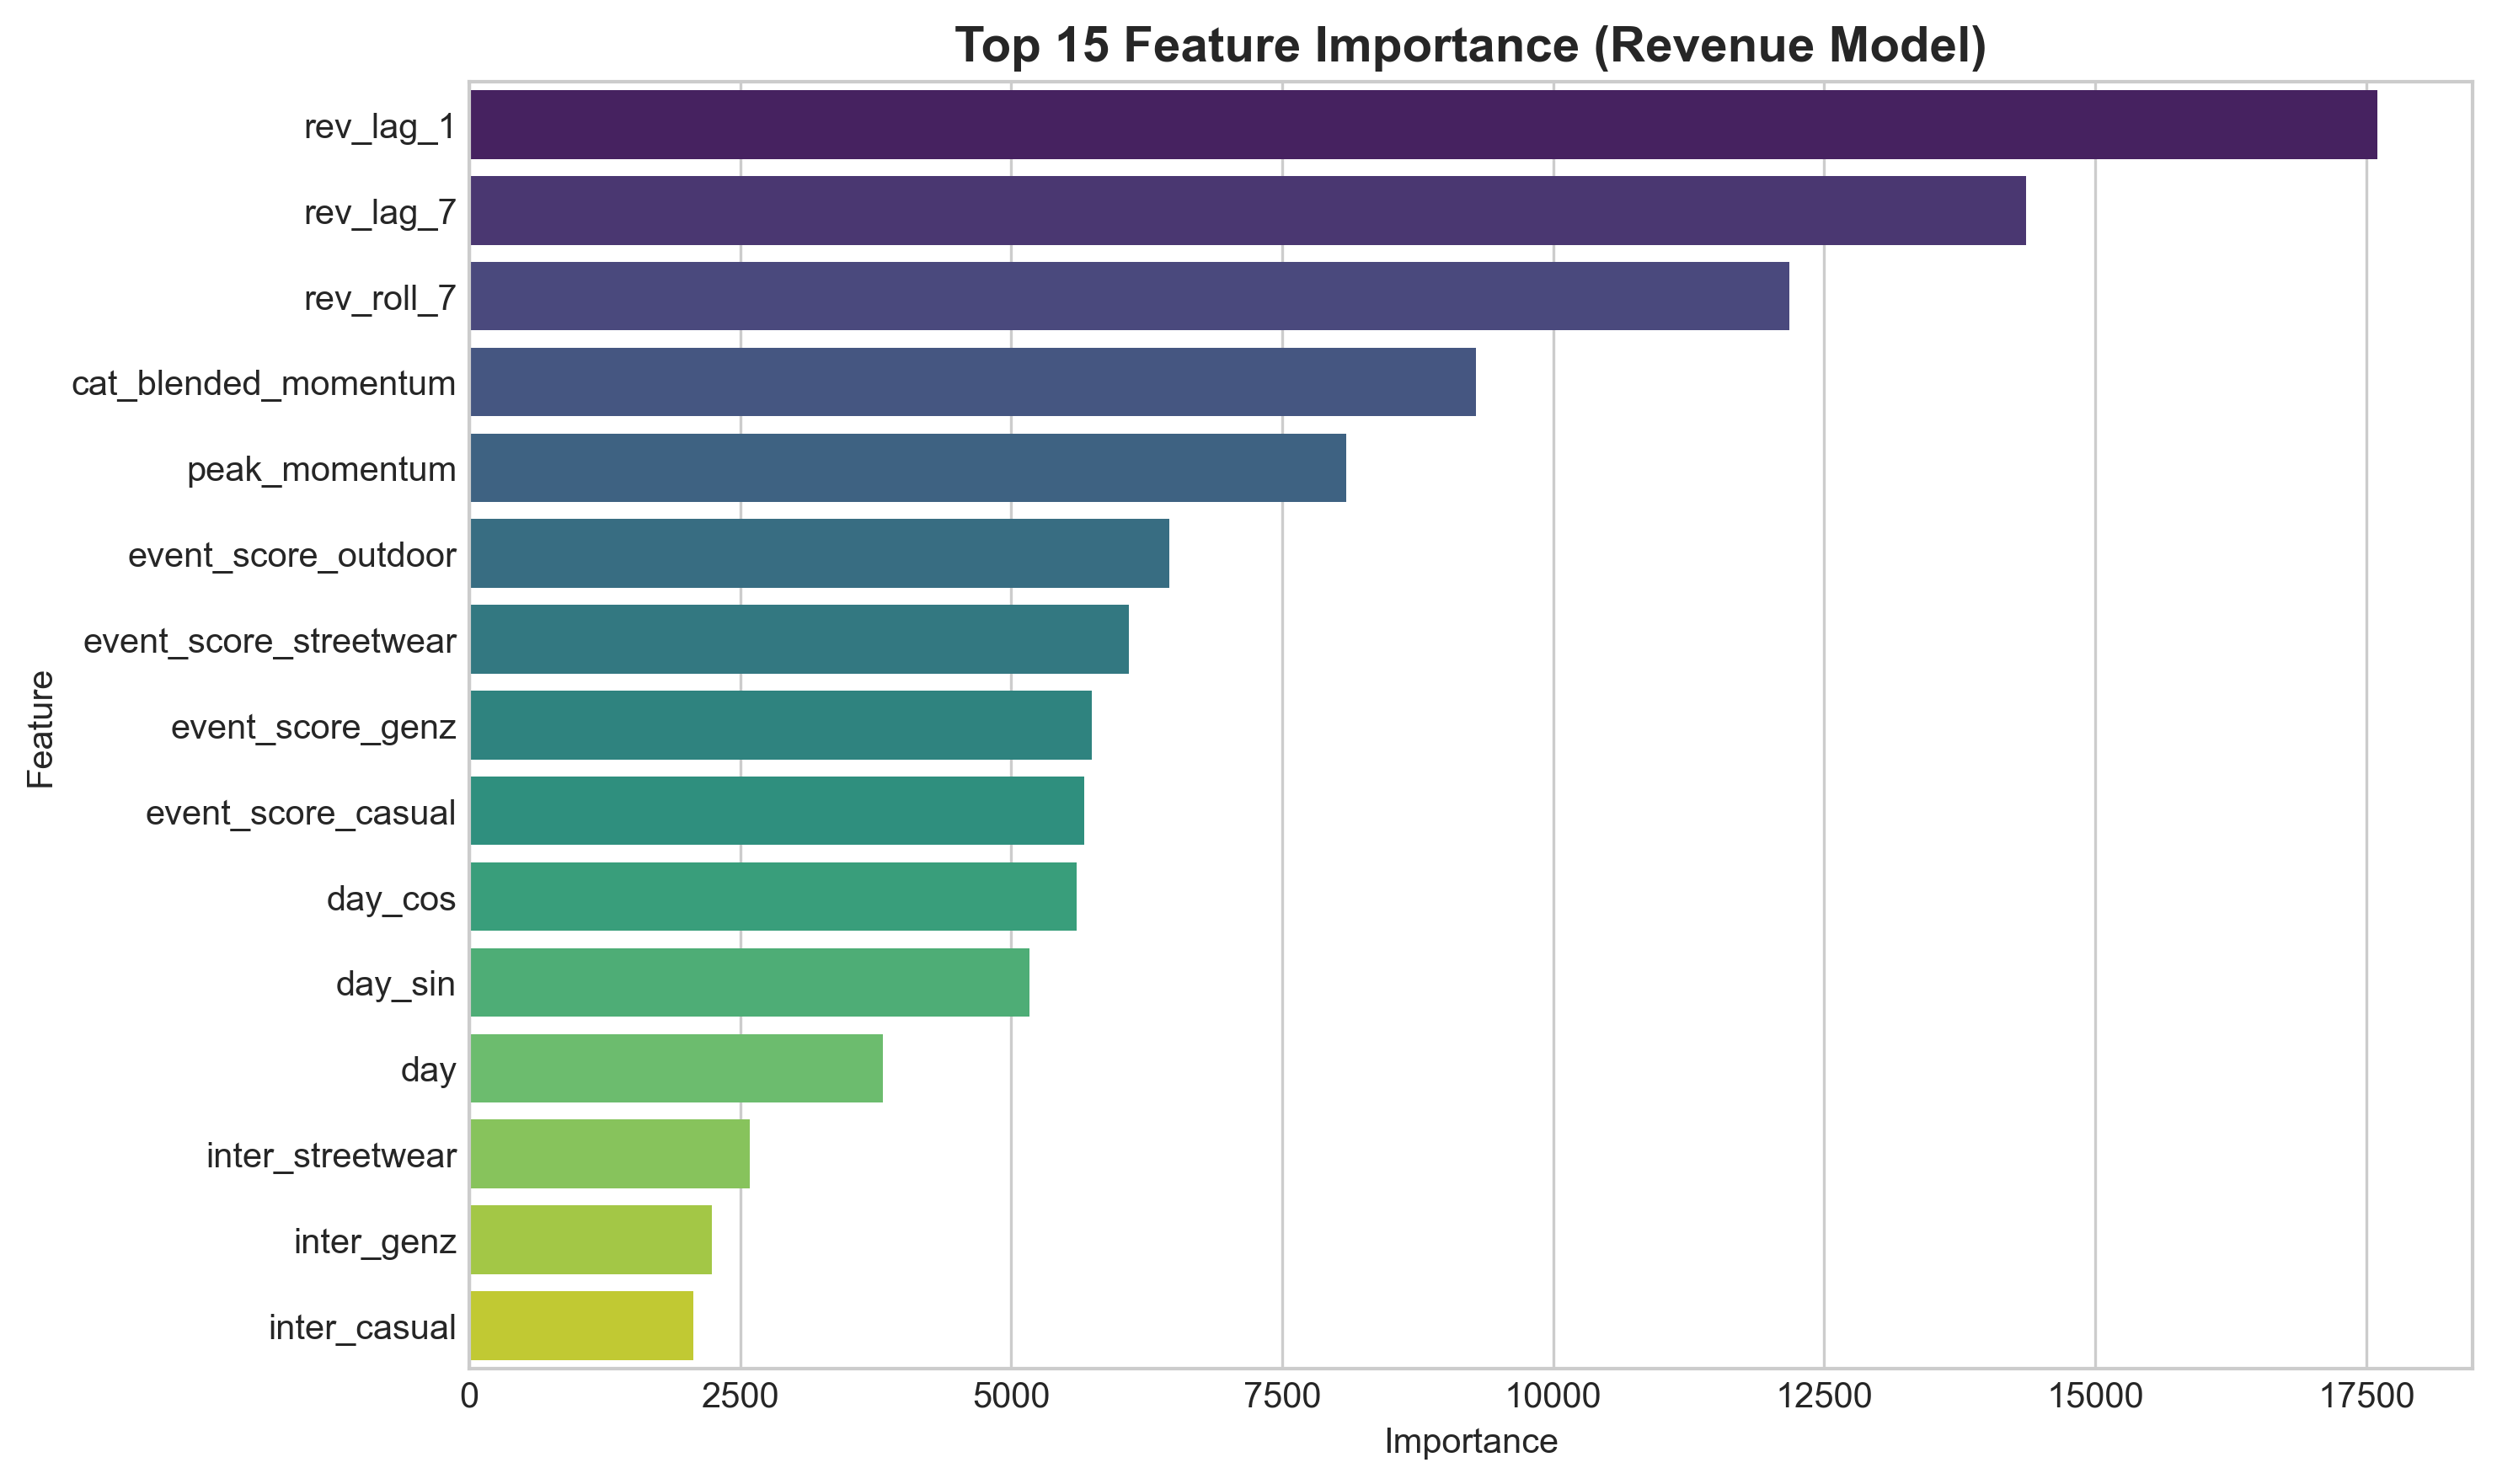
\includegraphics[width=\linewidth]{feature_importance}
    \caption{Feature Importance theo Gain.}
    \label{fig:fi}
  \end{subfigure}
  \caption{(Trái) Dự báo bắt đúng xu hướng tổng thể nhưng còn lệch tại
    các đỉnh sự kiện. (Phải) Ba feature quan trọng nhất đều là
    lag/momentum -- thị trường phản ứng với lịch sử gần hơn là mùa vụ cố định,
    đây là lý do chúng tôi chọn kiến trúc Recursive thay vì Direct.}
  \label{fig:model_results}
\end{figure}

% =========================================================
\section{Kết luận}
% =========================================================

Sự sụp đổ năm 2019 không đến từ việc thiếu hàng hay thiếu khách -- tỷ lệ lấp đầy đơn hàng đạt gần 96\% nhưng
lý do hoàn trả do sai kích cỡ và mô tả không đúng chiếm đến 52.6\%, khiến tỷ lệ giữ chân khách năm thứ 2 rớt xuống mức báo động 9.4\%. Việc ứng dụng Chuẩn hóa tĩnh (Stationary Normalization)
kết hợp đánh trọng số theo giai đoạn thị trường giúp hệ thống thích nghi thành công với đứt gãy cấu trúc, đạt
MAE 684{,}330 (Weighted CV). Hướng tối ưu tiếp theo:
mô hình hóa các đợt tăng vọt doanh thu cục bộ trong tháng (intra-month spikes) và cập nhật lại chu kỳ mua sắm theo ngày trong tuần cho phù hợp với hành vi hiện hành.

\bibliographystyle{plain}
\begin{thebibliography}{9}
\bibitem{lgbm}
Ke, G. et al. (2017). \textit{LightGBM: A Highly Efficient Gradient Boosting Decision Tree}. NeurIPS.
\bibitem{recursive}
Ben Taieb, S. \& Hyndman, R. J. (2012). \textit{Recursive and direct multi-step forecasting}. Monash WP 19/2012.
\bibitem{stationary}
Oreshkin, B. N. et al. (2020). \textit{N-BEATS}. ICLR 2020.
\end{thebibliography}

\end{document}